%%%%%%%%%%%%%%%%%%%%%%%%%%%%%%%%%%%%%%%%%
% Beamer Presentation
% LaTeX Template
% Version 1.0 (10/11/12)
%
% This template has been downloaded from:
% http://www.LaTeXTemplates.com
%
% License:
% CC BY-NC-SA 3.0 (http://creativecommons.org/licenses/by-nc-sa/3.0/)
%
%%%%%%%%%%%%%%%%%%%%%%%%%%%%%%%%%%%%%%%%%

%----------------------------------------------------------------------------------------
%	PACKAGES AND THEMES
%----------------------------------------------------------------------------------------

\documentclass{beamer}

\mode<presentation> {

% The Beamer class comes with a number of default slide themes
% which change the colors and layouts of slides. Below this is a list
% of all the themes, uncomment each in turn to see what they look like.

%\usetheme{default}
%\usetheme{AnnArbor}
%\usetheme{Antibes}
%\usetheme{Bergen}
%\usetheme{Berkeley}
%\usetheme{Berlin}
%\usetheme{Boadilla}
%\usetheme{CambridgeUS}
%\usetheme{Copenhagen}
%\usetheme{Darmstadt}
%\usetheme{Dresden}
%\usetheme{Frankfurt}
%\usetheme{Goettingen}
%\usetheme{Hannover}
%\usetheme{Ilmenau}
%\usetheme{JuanLesPins}
%\usetheme{Luebeck}
\usetheme{Madrid}
%\usetheme{Malmoe}
%\usetheme{Marburg}
%\usetheme{Montpellier}
%\usetheme{PaloAlto}
%\usetheme{Pittsburgh}
%\usetheme{Rochester}
%\usetheme{Singapore}
%\usetheme{Szeged}
%\usetheme{Warsaw}

% As well as themes, the Beamer class has a number of color themes
% for any slide theme. Uncomment each of these in turn to see how it
% changes the colors of your current slide theme.

%\usecolortheme{albatross}
%\usecolortheme{beaver}
%\usecolortheme{beetle}
%\usecolortheme{crane}
%\usecolortheme{dolphin}
%\usecolortheme{dove}
%\usecolortheme{fly}
%\usecolortheme{lily}
%\usecolortheme{orchid}
%\usecolortheme{rose}
%\usecolortheme{seagull}
%\usecolortheme{seahorse}
%\usecolortheme{whale}
%\usecolortheme{wolverine}

%\setbeamertemplate{footline} % To remove the footer line in all slides uncomment this line
%\setbeamertemplate{footline}[page number] % To replace the footer line in all slides with a simple slide count uncomment this line

%\setbeamertemplate{navigation symbols}{} % To remove the navigation symbols from the bottom of all slides uncomment this line
}

\usepackage{graphicx} % Allows including images
\usepackage{booktabs} % Allows the use of \toprule, \midrule and \bottomrule in tables
\usepackage{multirow}
\usepackage{adjustbox}
\usepackage{array}
\newcommand{\xmark}{\textcolor{red}{\text{\sffamily X}}}
\newcommand{\cmark}{\textcolor{green}{\checkmark}}
\newcommand{\tr}{\text{tr}}
\newcommand{\E}{\textbf{E}}
\newcommand{\diag}{\text{diag}}
\newcommand{\argmax}{\text{argmax}}
\newcommand{\argmin}{\text{argmin}}
\newcommand{\Cov}{\text{Cov}}
\newcommand{\Vol}{\text{Vol}}

%----------------------------------------------------------------------------------------
%	TITLE PAGE
%----------------------------------------------------------------------------------------


\title[Informal]{The geometry of human perception: RSA and multivariate models}

\author{Charles Zheng} % Your name
\institute[Stanford] % Your institution as it will appear on the bottom of every slide, may be shorthand to save space
{Stanford University}
\date{\today} % Date, can be changed to a custom date

\begin{document}

\begin{frame}
\titlepage % Print the title page as the first slide
(Joint work with Yuval Benjamini and Oluwasanmi Koyejo)
\end{frame}

\begin{frame}
\frametitle{Overview}
\noindent\emph{fMRI Background:}
\begin{itemize}
\item Nonparametric approaches: RSA.
\item Parametric approach: Multivariate linear model.
\end{itemize}
\noindent\emph{Questions:}
\begin{itemize}
\item Defining the RSA null and alternative hypotheses.
\item Scientific interpretation of RSA results.
\item Sensitivity to preprocessing choices.
\end{itemize}
\noindent\emph{Proposed Projects:}
\begin{itemize}
\item Distribution-induced distance.
\item Parametric RSA.
\end{itemize}
\end{frame}

\begin{frame}
\frametitle{Representation similarity analysis (RSA)}
\begin{itemize}
\item Framework for studying how mental objects are represented in the brain,
via brain activity (measured by fMRI, EEG) or behavior.
\item Compare different brain regions or imaging modalities within a single subject, or compare multiple subjects.
\end{itemize}
\begin{center}
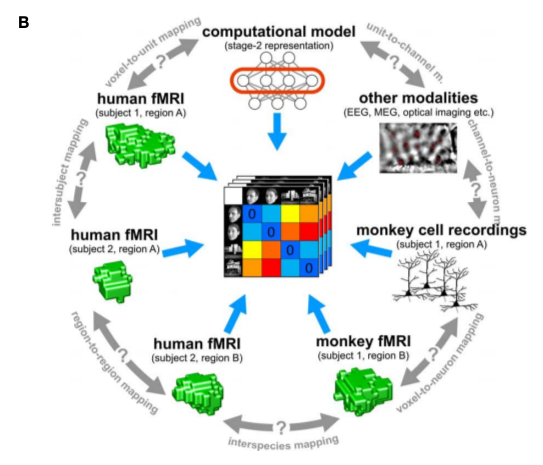
\includegraphics[scale = 0.3]{k08_b.png}
\end{center}
\end{frame}

\begin{frame}
\frametitle{A typical RSA experiment}
An experiment which demonstrates which regions of the brain differentiate between faces and objects.
\begin{center}
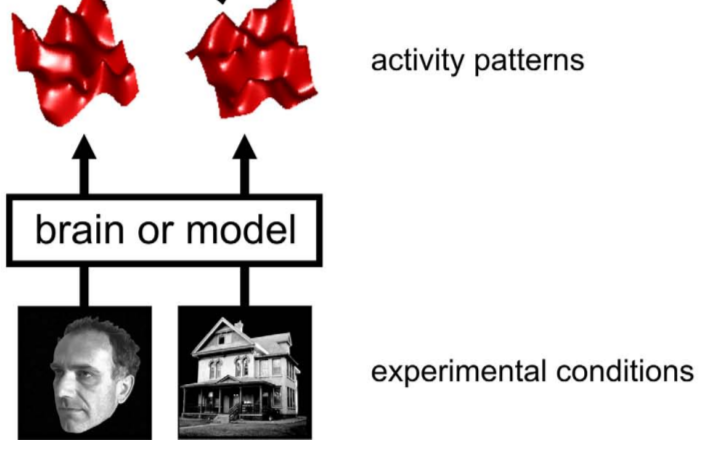
\includegraphics[scale = 0.3]{k08_step1.png}
\end{center}
Step 1: Present the subject with visual stimuli, pictures of faces and houses.
Record the subject's brain activity in the fMRI scanner.
\end{frame}

\begin{frame}
\frametitle{A typical RSA experiment}
Step 2a: Process the data, and represent the brain activity of the subject for the $i$th stimulus as a real vector $y_i$.
Form matrix of distances between $y_i$ and $y_j$, the \emph{representation distance matrix} (RDM).
\begin{center}
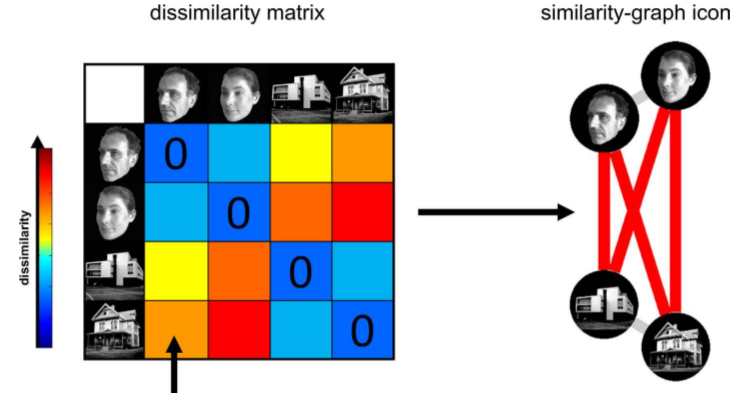
\includegraphics[scale = 0.3]{k08_step2.png}
\end{center}
Step 2b: Assess statistical significance of distances to form similarity graph.
\end{frame}

\begin{frame}
\frametitle{A typical RSA experiment}
Step 3: Compare similarity graphs between different brain regions.
\begin{center}
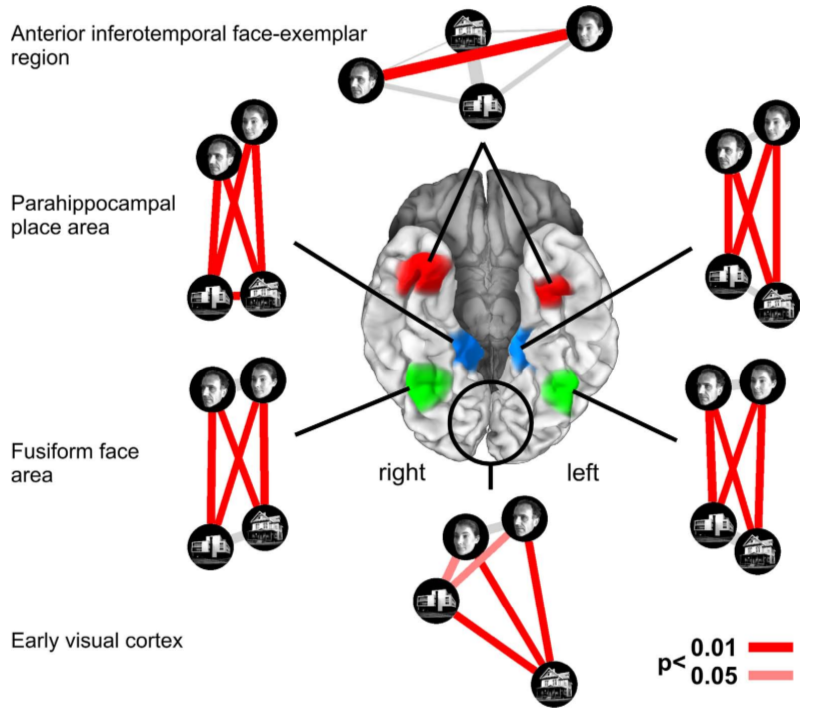
\includegraphics[scale = 0.2]{k08_step3.png}
\end{center}
Step 4: Draw scientific conclusions.  (Step 5: Profit!!..?)
\end{frame}

\begin{frame}
\frametitle{Details of RSA}
\begin{itemize}
\item Core methodology presented by Kriegeskort et al (2008) and extended by others.
\item Suppose each of the stimuli have $r$ repeats, the responses for stimulus $i$ are $y_i^1,\hdots, y_i^r$,
and the average over the repeats as $\bar{y}_i$.
\item The representation distance matrix is computed as
\[
D_{ij} = d(\bar{y}_i, \bar{y}_k)
\] 
where $d$ may be Euclidean distance or correlation distance.
\end{itemize}
\end{frame}

\begin{frame}
\frametitle{Details of RSA}
\begin{itemize}
\item Now let $D^A$, $D^B$ be \emph{two} such distance matrices, e.g. two regions from same subject, or same region in two subjects.
\item \emph{Estimation.} One can define a distance metric  $\mathfrak{d}$ \emph{between} distance matrices, e.g. the Spearman correlation between the entries of $D^A$ and $D^B$,
and estimate
\[
\mathfrak{d}(D^A, D^B).
\]
\item \emph{Testing.}  One can test:
\begin{itemize}
\item \emph{Independence} of $D^A, D^B$.
\item \emph{Equality} $D^A = D^B$.
\item Which of $D^A, D^B$ is closer to a reference distance matrix $D^0$.
\end{itemize}
\end{itemize}
\end{frame}


\begin{frame}
\frametitle{Comparison to parametric approach}
\begin{itemize}
\item RSA is a ``nonparametric'' approach, because stimuli are treated as discrete classes.
\item In contrast, one could consider presenting stimuli which are parameterized.
\item Example: present the subject with gratings of varying orientation.  Orientation $x$ is parameter.
\end{itemize}
\begin{center}
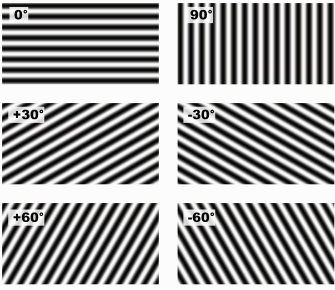
\includegraphics[scale = 0.2]{grating_angle.png}
\end{center}
\end{frame}

\begin{frame}
\frametitle{Example of parametric approach: natural images}
\begin{center}
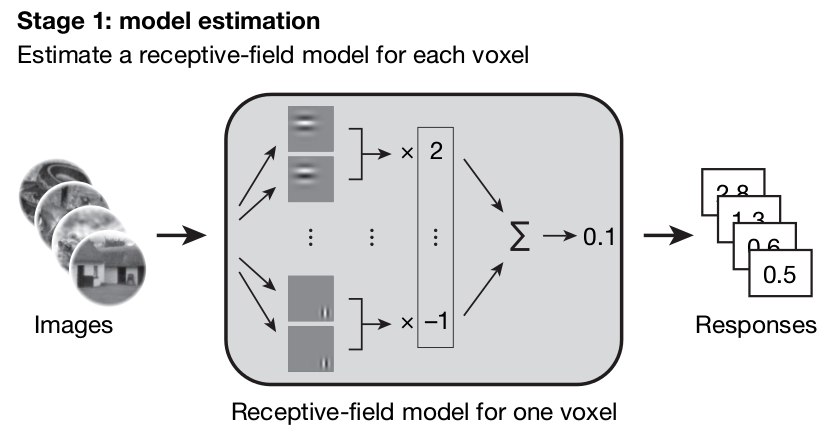
\includegraphics[scale = 0.2]{kay_stage1.png}
\end{center}
\begin{itemize}
\item Kay et al (2008) parameterize natural images using \emph{Gabor filters}.
\item Let $x_i$ be the vector of 10000 Gabor filter coefficients for a natural image.
Let $y_i$ be the vector of 20000 individual voxel responses.
\item Kay fits a model of the form
\[
y_i = B^T x_i + \epsilon_i
\]
where $B$ is a 10000 x 20000 coefficient matrix, and $\epsilon_i$ is vector-valued noise with covariance $\Sigma$.
\end{itemize}
\end{frame}

\begin{frame}
\frametitle{Comparison of parametric and nonparametric approaches}
Nonparametric: RSA
\begin{tabular}[t]{|p{5cm}|p{5cm}|}
\firsthline
Pros & Cons\\ \hline
Compare across subjects, regions, modalities & Can't generalize to new stimuli\\
\hline
\end{tabular}

\vspace{0.2in}
Parametric: Regression
\begin{tabular}[t]{|p{5cm}|p{5cm}|}
\firsthline
Pros & Cons\\ \hline
Predictive and descriptive power & Requires knowing featurization \emph{a priori}\\
\hline
\end{tabular}

\vspace{0.2in}
See also Kriegeskorte and Bandettini (2007) ``Analyzing for information...''
\end{frame}

\section{Questions}

\begin{frame}
\frametitle{Defining the RSA null}
\begin{itemize}
\item Consider the problem of testing \emph{equality} $D^A = D^B$.
\item Obviously, the matrices $\hat{D}^A$ and $\hat{D}^B$ computed from data will \emph{not} be equal!
\item We need to define the \emph{population} parameters $D^A$, $D^B$ in order to have a well-defined test.
\end{itemize}
\end{frame}

\begin{frame}
\frametitle{Possible definitions of population distance matrices}
\begin{itemize}
\item Option 1: Let $\mu_i = \E[y_i]$ averaged over repetitions, then define the population parameter as
\[
D_{ij} = d(\mu_i, \mu_j)
\]
This option \emph{ignores noise}
\item Option 2: Define
\[
D_{ij} = \E[d(y_i^1, y_j^1)]
\]
where the average is over a single repetition.  This option \emph{includes the effect of noise} in the population parameter.
Also, $\hat{D}_{ij}$ is an unbiased estimator of $D_{ij}$ if only one repeat per stimulus is used.
\end{itemize}
\end{frame}

\begin{frame}
\frametitle{Defining the RSA null}
\begin{itemize}
\item The most commonly used test in RSA is a test of \emph{independence} $D^A$ of $D^B$.
\item This approach was suggested by Kriegeskorte (2008) and is well-established in ecological data analysis.
\item Implemented via Mantel and partial Mantel tests (which use permutation).
\item However, how can we define the null hypothesis of
  ``independence''??  No matter how the \emph{population} matrices
  $D^A$ and $D^B$ are defined, they are \emph{deterministic} and hence
  it does not make sense to consider them \emph{dependent}.
\item Perhaps you could test if the entry-wise correlation is zero??
\end{itemize}
\end{frame}

\begin{frame}
\frametitle{Scientific interpretation of RSA results}
\begin{center}
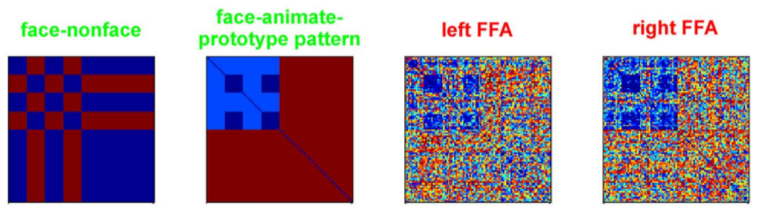
\includegraphics[scale = 0.3]{k08_classes.png}
\end{center}

A rejection of the independence null between $D^A$ and $D^B$ is taken to mean that outputs $A$ and $B$ are `related.'
For instance, $D^A$ might be the response from a subject's brain region, and $D^B$ is a 0-1 matrix reflecting \emph{a priori} class membership.
Rejection is taken to mean that the region $A$ have differential activation depending on the classes represented $D^B$.
\end{frame}

\begin{frame}
\frametitle{Scientific interpretation of RSA results}

What does it mean to reject $D^A = D^B$?
We can conclude that the means $\mu_i^A$ are \emph{not} related to the means $\mu_i^B$
by a scaling factor and orthogonal rotation:
\[
\mu_i^A \neq k H \mu_i^B
\]
where $H^T H = I$.

But we have not ruled out the possibility that $\mu_i = \psi(\mu_j)$ for some bijection.
Hence we can only draw a very weak conclusion about the difference between $D^A$ and $D^B$.
\end{frame}

\begin{frame}
\frametitle{Sensitivity to preprocessing choices}
Even given the same raw data, there are a variety of choices for representing the response vectors $y_i$:
\begin{itemize}
\item Volumetric (voxels) vs surface-based coordinates;
\item Voxel size and centering;
\item Smoothing;
\item Image registration;
\item Representation of data via function basis.
\end{itemize}

The resulting distance matrix $D_{ij}$ depends on the above choices.
\end{frame}

\section{Proposed Projects}

\begin{frame}
\frametitle{Distribution-induced distance}
A new definition for the \emph{representation dissimilarity matrix} which:
\begin{itemize}
\item Allows more natural interpretation of the null $D^A = D^B$;
\item Is nearly invariant to smoothing, registration, use of function bases;
\item Downside: may be harder to estimate.
\end{itemize}
\end{frame}

\begin{frame}
\frametitle{Distribution-induced distance: motivation}
Consider two stimuli $x_1$ and $x_2$ to be \emph{distant} if the \emph{response distributions} are statistically distant,
or \emph{close} if their response distributions overlap.
\begin{center}
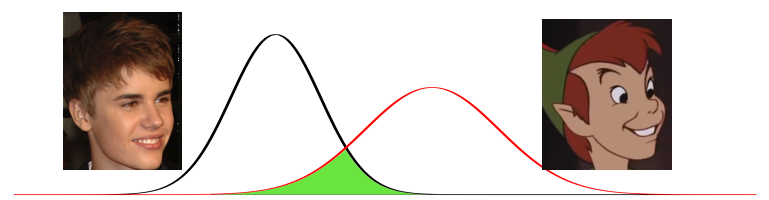
\includegraphics[scale = 0.3]{similarity.png}
\end{center}
Note that the definition not only depends on the difference in \emph{means} but also depends on the \emph{noise distribution}.
\end{frame}

\begin{frame}
\frametitle{Distribution-induced distance: definition}
\begin{itemize}
\item Let $\mathcal{F}_x$ denote the distribution of the reponse $y$ conditional on the stimulus $x$.
\item Define the dissimilarity matrix
\[
D_{ij} = \mathbb{D}(\mathcal{F}_{x_i}; \mathcal{F}_{x_j})
\]
where $\mathbb{D}$ is a measure of distance or divergence between probability measures.
\item Example: if $y$ is conditionally multivariate normal, with covariance $\Sigma$ not depending on $x$, then
\[
D_{ij} = \frac{1}{2}(\E[y|x_i] - \E[y|x_j])^T \Sigma^{-1} (\E[y|x_i] - \E[y|x_j])
\]
for either $\mathbb{D}=$ KL divergence or Hellinger distance.
\end{itemize}
\end{frame}

\begin{frame}
\frametitle{Distribution-induced distance: properties}
\begin{itemize}
\item Invariance under bijections: Let $\tilde{y} = \psi(y)$ for some
  bijection $\psi$.  Then if $\mathcal{F}_x^{\tilde{y}}$ denotes the
  conditional distribution of $\tilde{y}$ given $x$, we have
\[
\mathbb{D}(\mathcal{F}_x^y, \mathcal{F}_{x'}^y) = \mathbb{D}(\mathcal{F}_x^{\tilde{y}}, \mathcal{F}_{x'}^{\tilde{y}})
\]
for any $f$-divergence $\mathbb{D}$.
\item Near-invariance under sampling.  Suppose the `true' brain
  activity is represented by a random process $f$, and let
  $\mathcal{F}_x$ denote its conditional distribution given $x$.
  Define the vector $y$ as the values of linear functionals
  $\Lambda_1,\hdots, \Lambda_q$ evaluated on $f$.  This corresponds to
  taking $y$ based on binning the signal $f$ or taking coefficients of
  $f$ from a function basis.  Then, supposing $\Lambda_1,\hdots$ is
  `dense'
\[
\lim_{q \to \infty} \mathbb{D}(\mathcal{F}_x^y, \mathcal{F}_{x'}^y) = \mathbb{D}(\mathcal{F}_x^f, \mathcal{F}_{x'}^f).
\]
\end{itemize}
\end{frame}

\begin{frame}
\frametitle{Distribution-induced distance: consequences}
What does it mean to reject $D^A = D^B$?

Invariance under bijections means that $y^A$ and $y^B$ are different
in a stronger sense: not only is it the case that $y^A$ and $y^B$ have
different distributions, but we can also rule out the possibility that
$y^A$ and $y^B$ are related by maps $\psi^{A\to B}$ and $\psi^{B \to
  A}$ where
\[
y^A|x \stackrel{D}{=} \psi^{A\to B}(y^B)|x
\]
\[
y^B|x \stackrel{D}{=} \psi^{B\to A}(y^B)|x.
\]

Hence the conditional distributions of $y^A$ and $y^B$ \emph{carry different information.}
\end{frame}

\begin{frame}
\frametitle{Distribution-induced distance: consequences}
Near-invariance under sampling means that the population distances
$D_{ij}$ are robust to choices in coordinates, smoothing, etc,
\emph{supposing that sufficiently many dimensions are used}.

This is because any choice of extracting the vector $y$ from the 3-dimensional function-valued signal
amounts to a choice of linear functionals $\Lambda_1,\hdots, \Lambda_q$.  For example:
\begin{itemize}
\item Voxels + smoothing: each coordinate of $y_i$ takes the form
\[
y_i = \int \phi(z - c_i) f(z) fz
\]
where $\phi$ is a gaussian kernel, $c_i$ is the center of the $i$th voxel and $f(z)$ is the ``true signal''
\item Function basis:
\[
y_i = \int \phi_i(z) f(z) fz
\]
where $\{\phi_1,\hdots, \phi_q\}$ is the function basis.
\end{itemize}
\end{frame}

\begin{frame}
\frametitle{Parametric RSA}
\begin{itemize}
\item Combine the parametric approach of multivariate regression with RSA.
\item Model:
\[
y \sim N(B^T x, \Sigma).
\]
\item The distribution-induced metric is therefore
\[
D(x_i, x_j) = (x_i - x_j)^T B \Sigma^{-1} B^T (x_i - x_j).
\]
\end{itemize}
\end{frame}

\begin{frame}
\frametitle{Parametric RSA}
\[
y \sim N(B^T x, \Sigma)
\]
\[
D(x_i, x_j) = (x_i - x_j)^T B \Sigma^{-1} B^T (x_i - x_j)
\]
\begin{itemize}
\item Since all information about the distance is captured by the matrix $M = B\Sigma^{-1}B^T$, instead of testing
\[
D^A = D^B
\]
we can test
\[
M^A = M^B.
\]
\item We can compare two datasets with non-overlapping stimuli
\item The approach is scalable in the number of distinct stimuli,
  since the size of $M^A$, $M^B$ only depend on the number of
  \emph{features} rather than the number of stimuli
\end{itemize}
\end{frame}

\begin{frame}
\frametitle{References}
\begin{itemize}
\item Kriegeskorte, N. (2008). Representational similarity analysis – connecting the branches of systems neuroscience. Frontiers in Systems Neuroscience
\item Kriegeskorte, N., \& Bandettini, P. (2007). Analyzing for information, not activation, to exploit high-resolution fMRI. NeuroImage, 38(4), 649–662. doi:10.1016/j.neuroimage.2007.02.022
\item Kay, K. N., Naselaris, T., Prenger, R. J., \& Gallant, J. L. (2008). Identifying natural images from human brain activity. Nature, 452(March), 352–355. doi:10.1038/nature06713
\item Guillot, G., \& Rousset, F. (2013). Dismantling the Mantel tests. Methods in Ecology and Evolution, 4(4), 336–344. doi:10.1111/2041-210x.12018
\item Cole, M. W., Reynolds, J. R., Power, J. D., Repovs, G., Anticevic, A., \& Braver, T. S. (2013). Multi-task connectivity reveals flexible hubs for adaptive task control. Nature Neuroscience, 16(9), 1348–1355. doi:10.1038/nn.3470
\end{itemize}
\end{frame}

\end{document}












